\section{Results}\label{sec:results}

\subsection{Accuracy and the set of equally accurate models}

The most accurate default model is an unconstrained LightGBM model at every
date, with held-out AUC between \num{res.auc.min} and \num{res.auc.max}.
Accuracy differences across the grid are small next to the sampling error of
any one model's held-out log loss. The set therefore holds a median of
\num{res.set.size.median} of the \num{const.n_models} models (between
\num{res.set.size.min} and \num{res.set.size.max}), about \num{res.mono.share}\%
of them monotone-constrained. The spline logit is in the set only at the five
earliest dates. \Cref{fig:cloud} plots, at six dates, every model's held-out
log loss above the best (in standard errors) against its allowance relative
to the best. Within the shaded band of equal accuracy, allowances spread
widely.

\begin{figure}[t]
\centering
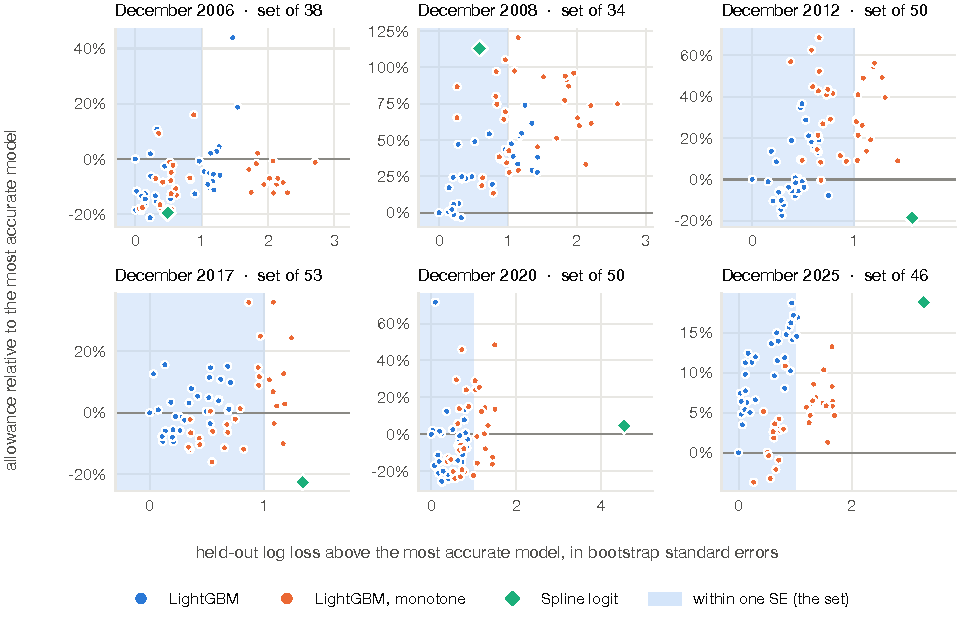
\includegraphics[width=\linewidth]{figures/cloud.pdf}
\caption{Accuracy and allowance for all \num{const.n_models} default models at
six reporting dates. Horizontal: held-out log loss above the most accurate
model, in bootstrap standard errors of that model's log loss. Vertical:
lifetime allowance relative to the most accurate model's. The shaded band is
the set of equally accurate models.}
\label{fig:cloud}
\end{figure}

\subsection{How far the allowance moves}\label{sec:sampling}

\Cref{fig:allowance}A shows the allowance across time. The most accurate
model's lifetime allowance runs from \num{res.best_rate.min}\% of balance to
\num{res.best_rate.max}\% (December \num{res.best_rate.max_year}). The range
across the set, as a share of the most accurate model's allowance, has a
median of \num{res.rel.median}\% across dates, from \num{res.rel.min}\% (December
\num{res.rel.min_year}) to \num{res.rel.max}\% (December \num{res.rel.max_year}).
Scaled to Freddie Mac's whole non-defaulted active book in the standard dataset, the range is
\num{res.usd.median} billion dollars at the median date and
\num{res.usd.max} billion dollars at December \num{res.usd.max_year}
(\cref{fig:dollars}). Drawing the 200{,}000 scored loans is not the source:
the bootstrap standard error of the allowance from that sampling has a median
of \num{res.samp_se.median_bp} basis points of balance, against a median range of
\num{res.range_bp.median} basis points. \Cref{tab:bydate} in
\cref{app:bydate} gives every date.

\begin{figure}[t]
\centering
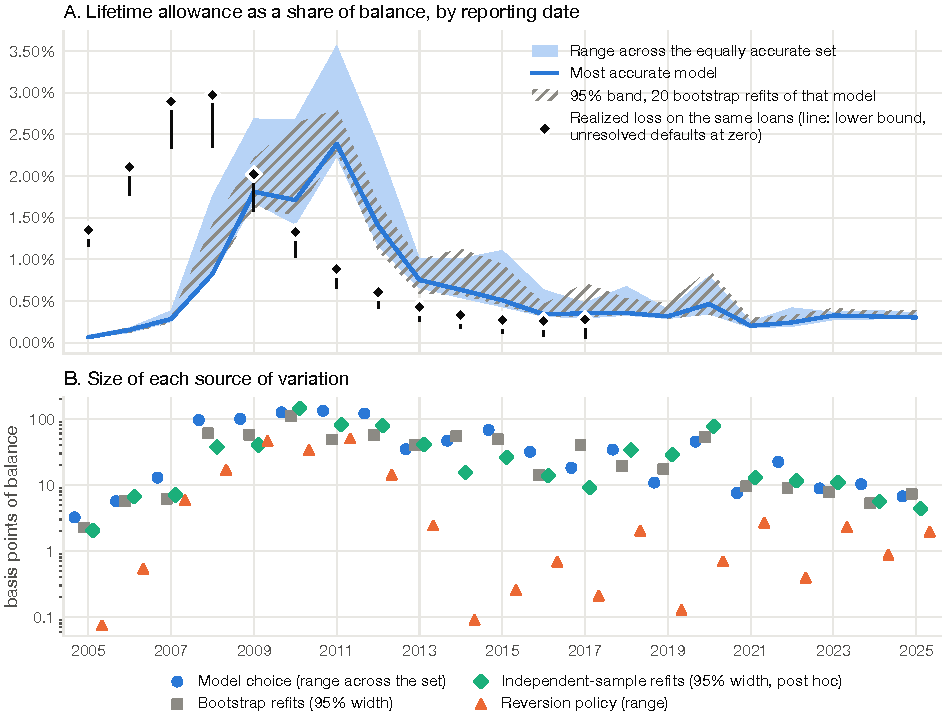
\includegraphics[width=\linewidth]{figures/allowance.pdf}
\caption{A: lifetime allowance as a share of the scored loans' balance, under
the primary forecast path and one-year straight-line reversion. The band is
the range across the set of equally accurate models; the hatched band the
central 95\% of 20 bootstrap refits of the most accurate configuration.
Diamonds: realized credit losses on the same loans for dates with at least
eight years of outcomes; the line below each diamond runs to the lower bound
in which defaults still unresolved in June 2026 carry no loss. B: the sources
of variation in basis points of balance (log scale); the independent-sample
refits of \cref{sec:refits} were added after the results.}
\label{fig:allowance}
\end{figure}

\begin{figure}[t]
\centering
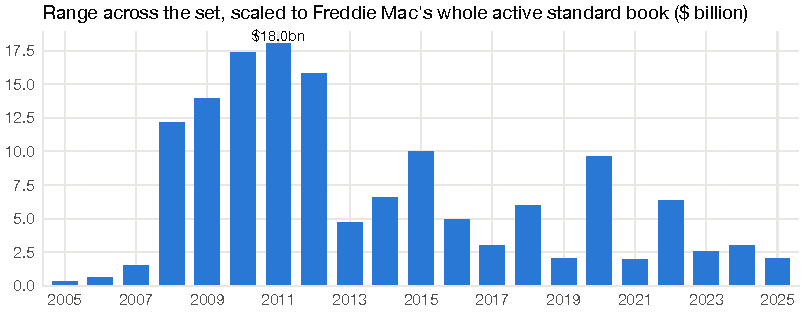
\includegraphics[width=\linewidth]{figures/dollars.pdf}
\caption{Range of the allowance across the set of equally accurate models,
multiplied by the balance of every loan active in Freddie Mac's standard
dataset at each year-end.}
\label{fig:dollars}
\end{figure}

\subsection{The six predictions}

\begin{table}[t]\centering\small
\caption{The six predictions recorded before the data were opened, as tested.}\label{tab:hyp}
\begin{tabular}{llll}\toprule
& Prediction & Evidence & Verdict \\ \midrule
H1 & Model choice $>$ refit noise & 13 of 21 dates & Holds \\
H2 & Model choice $\ge$ reversion range (1 vs 3 years) & 21 of 21 dates & Holds \\
H3 & Relative range larger at 2006 and 2007 & 37\%, 46\% vs 56\% & \textbf{Fails} \\
H4 & Monotone family narrower & 12 of 21 dates & Holds \\
H5 & Realized loss inside the range at $<$ half & 1 of 13 dates & Holds \\
H6 & Stage flips $>$ refit flips & 17 of 21 dates & Holds \\
\bottomrule\end{tabular}
\end{table}


\Cref{tab:hyp} summarises the verdicts. Two of them, H1 and H6, depend on
how the tests were built, and \cref{sec:likeforlike} reports like-for-like
versions.

\paragraph{H1 (model choice exceeds refit noise) \num{H1.verdict}.} The
range across the set exceeds the 95\% width of 20 bootstrap refits at
\num{H1.n} of \num{const.n_dates} dates, with a median ratio of
\num{res.ratio_refit.median}. Training noise is large in its own right: at
several dates refitting the best configuration on resampled loans moves the
allowance by more than half its level (\cref{fig:allowance}A). The bootstrap
refits the test uses are a weaker benchmark than the design intended,
however; \cref{sec:refits} shows that refits on independent samples, which do
not share that weakness, span at least as much as the set.

\paragraph{H2 (model choice rivals the reversion policy) \num{H2.verdict}.} At
\num{H2.n} of \num{const.n_dates} dates the range across the set is at least
the range across the three reversion policies, with a median ratio of
\num{res.ratio_policy.median}. Immediate and one-year straight-line reversion
give the same annual path (\cref{sec:method}), so this is the range between
one- and three-year reversion, and the discretion over the length of the
forecast period, which is not varied here, would add to it. The policy matters
most when the economy at $T$ is far from its long-run average: its range is a
median of \num{res.policy.rel.median1}\% of the allowance, but
\num{res.policy.rel.gfc.min}\% to \num{res.policy.rel.gfc.max}\% at the
year-ends 2008 to 2011, \num{res.policy.rel.2007}\% at December 2007 and
\num{res.policy.rel.2021}\% at December 2021. The choice among
equally accurate models matters at every date (\cref{fig:allowance}B).

\paragraph{H3 (the spread widens into stress) \num{H3.verdict}.} The relative
range is \num{H3.rel2006}\% at December 2006 and \num{H3.rel2007}\% at December
2007, below the \num{H3.median}\% median of the other dates (\cref{fig:relative}).
On the eve of the crisis the models' disagreement was ordinary in relative
terms. It is the level of the allowance that was badly wrong, and the
absolute range then grew with it: in dollars the spread was largest from 2008
to 2012 (\cref{fig:dollars}).

\begin{figure}[t]
\centering
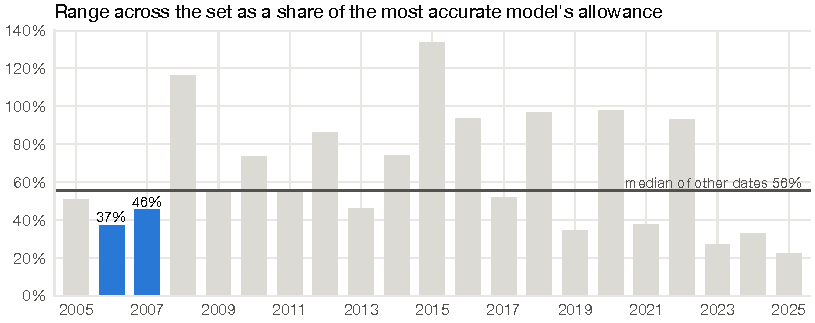
\includegraphics[width=\linewidth]{figures/relative.pdf}
\caption{Range across the set as a share of the most accurate model's
allowance. H3 predicted the two highlighted dates would exceed the median of
the others.}
\label{fig:relative}
\end{figure}

\paragraph{H4 (constraints narrow the spread) \num{H4.verdict}, narrowly.}
Within each family's own set, the monotone-constrained models have the
smaller relative range at \num{H4.n} of \num{const.n_dates} dates
(\cref{fig:families}A), one more than a majority. They do not narrow it on
average: the median relative range is \num{res.fam.mono.median}\% for the
constrained family and \num{res.fam.lgbm.median}\% for the unconstrained one.
Constraints that encode the
expected direction of credit risk do not reliably tie down the lifetime
allowance; most of the lifetime projection runs through inputs they leave free
(loan age, the macro path, the interaction of default with prepayment).
The two families' sets differ in size, and a range grows with the number of
models in it; comparing random subsets of equal size (added after the
results) leaves the verdict unchanged, with the constrained family narrower at
\num{p2.h4.n} dates and medians of \num{p2.h4.mono}\% and \num{p2.h4.lgbm}\%.

\paragraph{H5 (the range is not forecast uncertainty) \num{H5.verdict}.} For the
\num{H5.n_elig} reporting dates with at least eight years of outcomes
(\num{H5.first} to \num{H5.last}), realized credit losses on the scored loans lie
inside the set's range at \num{H5.inside} date (December 2009), and at none when
unresolved defaults are counted at zero. They lie above the range at the
\num{H5.above} dates from 2005 to 2008 and below it at the \num{H5.below} dates
from 2010 to 2017. Two caveats qualify the comparison. Outcomes are observed
only to June 2026, so the realized loss of the later portfolios is truncated
while the allowance is lifetime; the horizon-matched comparison (losses and
allowances both through 2025) puts realized losses inside the range at
\num{H5.inside25} dates. And a growing share of the later realized losses is
imputed for defaults not yet resolved (\cref{tab:decomp}, last column).

The range across equally accurate models says nothing about forecast error:
realized losses on the December 2006 portfolio were \num{res.miss2006} times
the top of the set's range, while the models agreed with one another far more
closely than with the outcome. \Cref{tab:decomp}, added after the results,
splits the miss for the most accurate model. Before the crisis the forecast
held each state's house-price growth at its December value (a median
\num{mac.hpi2005}\% a year at December 2005 and \num{mac.hpi2006}\% at December
2006) and the severity table reflected a benign history. Replacing the
forecast with the realized macro path raises the 2005--2008 allowances by a
factor of \num{dec.path.min} to \num{dec.path.max}. Replacing the severity
table with that of the defaults resolved by December 2019, after the crisis
losses and before pandemic forbearance, raises them by a further
\num{dec.lgd19.min} to \num{dec.lgd19.max} times (column 3). The result is
within \num{dec.lgd19.short.max}\% of realized losses at 2005, 2007 and 2008
and \num{dec.lgd19.over2006}\% above them at 2006. The default model itself was
not the main problem: on the realized path its mean lifetime PD is
\num{pd.pre.min} to \num{pd.pre.max} times the share of loans that actually
defaulted at the four pre-crisis dates. The miss came from the forecast and
from severities estimated on a benign history. The severity table of December
2025 (column 4) is a poorer guide to crisis losses, because it counts the
payoffs after pandemic-era ``defaults'' as zero-loss resolutions.

After the crisis the order reverses. The forecast held the high unemployment
of the years after 2009, and from December 2011 the realized path and the
2019 severities each lower the allowance, but column (3) still exceeds
realized losses at every date from 2010 to 2017. The defaults are not the
reason: for the 2013 to 2017 portfolios the model's lifetime PD is only
\num{pd.late.min} to \num{pd.late.max} times the realized default share, which
the pandemic forbearance ``defaults'' inflate. Those defaults resolved with
little loss, which no severity table estimated before 2020 anticipates;
column (4) is closer to realized losses from 2010 to 2015, partly mechanically, since the
imputed part of realized loss is valued at much the same diluted severities.
With the realized macro path
in place of the forecast, the set's range widens to a median of
\num{res.realpath.rel.median}\% of the best model's allowance, so the models
disagree most when the economy moves outside the training data.

\begin{table}[t]\centering\footnotesize
\caption{Where the miss comes from (added after the results). Lifetime allowance of the most accurate model, \% of balance: (1) primary forecast and the severity table at $T$; (2) realized macro path, severity at $T$; (3) realized path and the severity table of defaults resolved by December 2019, before pandemic forbearance; (4) realized path and the table of defaults resolved by December 2025, which counts pandemic-era payoffs after default as zero-loss resolutions. Realized loss: recorded estimate, lower bound with unresolved defaults at zero, and the imputed share, valued at the severity of all resolutions through June 2026. Defaults: the model's mean lifetime PD on the realized path, and the share of loans that defaulted by June 2026.}\label{tab:decomp}
\setlength{\tabcolsep}{3.5pt}
\begin{tabular}{rrrrrrrrrr}\toprule
& \multicolumn{4}{c}{Allowance} & \multicolumn{3}{c}{Realized loss} & \multicolumn{2}{c}{Defaults (\%)} \\
\cmidrule(lr){2-5}\cmidrule(lr){6-8}\cmidrule(lr){9-10}
Dec. & (1) & (2) & (3) & (4) & Est. & Lower & Imp.\,\% & PD & Actual \\ \midrule
2005 & 0.06 & 0.32 & 1.19 & 0.92 & 1.35 & 1.15 & 14 & 3.8 & 5.1 \\
2006 & 0.15 & 0.76 & 2.48 & 1.85 & 2.11 & 1.77 & 16 & 8.6 & 6.3 \\
2007 & 0.28 & 0.74 & 2.24 & 1.75 & 2.90 & 2.34 & 19 & 6.6 & 7.6 \\
2008 & 0.83 & 1.06 & 2.42 & 1.91 & 2.98 & 2.34 & 22 & 7.4 & 7.8 \\
2009 & 1.81 & 1.59 & 2.19 & 1.78 & 2.02 & 1.57 & 22 & 6.4 & 6.3 \\
2010 & 1.71 & 1.74 & 1.91 & 1.57 & 1.33 & 1.02 & 23 & 5.6 & 4.9 \\
2011 & 2.39 & 1.50 & 1.47 & 1.19 & 0.88 & 0.65 & 27 & 4.5 & 3.9 \\
2012 & 1.41 & 1.12 & 1.06 & 0.84 & 0.61 & 0.41 & 32 & 3.5 & 3.4 \\
2013 & 0.75 & 0.63 & 0.60 & 0.45 & 0.43 & 0.26 & 40 & 2.4 & 3.0 \\
2014 & 0.63 & 0.52 & 0.49 & 0.35 & 0.33 & 0.17 & 50 & 2.2 & 2.7 \\
2015 & 0.51 & 0.44 & 0.41 & 0.28 & 0.27 & 0.10 & 62 & 2.0 & 2.6 \\
2016 & 0.34 & 0.31 & 0.29 & 0.20 & 0.26 & 0.07 & 75 & 1.5 & 2.8 \\
2017 & 0.35 & 0.33 & 0.32 & 0.20 & 0.28 & 0.04 & 85 & 1.9 & 2.9 \\
\bottomrule\end{tabular}
\end{table}


\paragraph{H6 (staging flips) \num{H6.verdict}.} At \num{H6.n} of
\num{const.n_dates} dates more loans change IFRS 9 stage across the set than
across the refits, but the medians are almost equal: \num{res.flip.median}\% of
loans across the set and \num{res.flip_refit.median}\% across the refits
(\cref{fig:families}B). The prediction holds as recorded, but the
like-for-like comparisons of \cref{sec:refits} contradict the reasoning
behind it: refits change at least as many loans' stage as model choice. The share of loans in stage 2 under the best model
runs from \num{res.stage2.min}\% to \num{res.stage2.max}\%. Many loans sit near
the twice-the-origination-PD threshold, so any model change moves some of them
across it.

\begin{figure}[t]
\centering
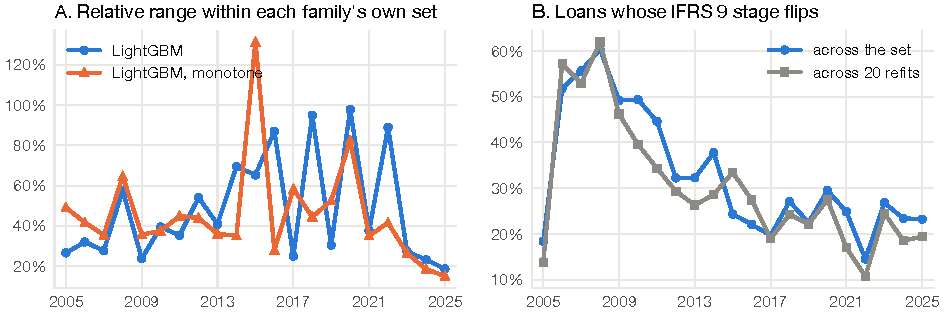
\includegraphics[width=\linewidth]{figures/families_stages.pdf}
\caption{A: H4, the relative range within each LightGBM family's own set of
equally accurate models. B: H6, the share of scored loans whose IFRS 9 stage
(lifetime PD more than twice its origination value) differs between at least
two models of the set, and between at least two of the 20 refits.}
\label{fig:families}
\end{figure}

\subsection{Refit noise, like for like (added after the results)}\label{sec:likeforlike}\label{sec:refits}

H1 and H6 as recorded have two weaknesses, both found after the results.
First, they compare a range or a disagreement among about fifty set models
with a central interval or a disagreement among twenty refits, so both lean
towards the set. Second, the recorded refits fit on bootstrap resamples of the
training loans, implemented as integer case weights; a resample contains
about 63\% of the distinct loans, and LightGBM's minimum leaf size and row
subsampling count rows, not weights. The refits are less accurate than the
model they refit: their held-out log loss is a median \num{ph.rq.gap} standard
errors above the best model's, \num{ph.rq.gt1} of the \num{ph.rq.total} refits
(\num{ph.rq.gt1.share}\%) would fall outside the set's tolerance, and their
mean allowance exceeds the best model's at \num{ph.rq.above} of
\num{const.n_dates} dates (median \num{ph.rq.bias}\%).

Two analyses address this. Twenty models are drawn at random from the set,
and the best configuration is refitted on twenty random samples of the panel,
each the same size as its original fitting sample, with the same fitting and
early-stopping split and the same held-out loans for accuracy. These refits
are as accurate as the original to within a fraction of a standard error
(median gap \num{ph.rs.gap}), so each is a model the lender could have fitted
and kept. The samples are windows of a uniform loan-level draw. When the
sampling fraction is below 1/21, at the \num{ph.rs.disj.n} dates from December
\num{ph.rs.disj.first}, they are disjoint from one another and from the
original. At earlier dates neighbouring windows overlap, by up to
\num{ph.rs.mut.max}\% of their loans (December \num{ph.rs.mut.max_year}), and
share at most \num{ph.rs.ov.max}\% with the original on average. Overlap
narrows the refits' spread, so the comparison is cleanest at the disjoint
dates.

There, training-sample noise exceeds model choice: twenty refits span a median
\num{p2.disj.rsm}\% of the allowance against \num{p2.disj.lfl}\% for twenty set
models, and more at \num{ph.rs.disj.refitmore} of the \num{ph.rs.disj.n}
dates. Over all dates, including those where overlap holds the refits back,
the two are equal: medians of \num{ph.rs.rel.median}\% and \num{ph.lfl.rel.median}\%, with
the set's twenty wider at \num{ph.rs.n} of \num{const.n_dates} dates (median
ratio \num{ph.rs.ratio}). Rerun against these refits, the recorded H1 test
(the set's full range against the refits' central 95\% width) would hold at
\num{ph.rs.w95} dates. Bootstrap refits span a median \num{p2.boot.rel}\%, more
than the independent refits at only \num{p2.boot_gt_rsm} dates, so their flaw
is inaccuracy and bias rather than a wider spread. For staging the comparison
is one-sided: the independent-sample refits flip a median \num{ph.rs.flip}\%
of loans' IFRS 9 stage against \num{ph.H6.flipset}\% for twenty set models, and
fewer at only \num{ph.rs.flipmore} dates.

The training samples here are capped near five million loan-years, which is
\num{ph.frac.min}\% of the history available at December
\num{ph.frac.min_year}. Fitting on all of Freddie Mac's history would shrink
this noise. A bank fitting on its own, much smaller, book would face more.

\paragraph{Where the most accurate model sits.} The most accurate model is in
the lower part of the set's range: a median \num{p2.pos.median}\% of the way
from the lowest allowance to the highest, below the set's median at
\num{p2.below_median} of \num{const.n_dates} dates, though the set's median is
only a median \num{p2.median_gap}\% above it. The range is skewed upward, with a
few models giving much higher allowances. Across the set, held-out log loss
and allowance are positively rank-correlated at \num{p2.rho_set.pos} dates
(median Spearman correlation \num{p2.rho_set.median}): the more accurate
models give lower allowances. Across the twenty refits of one configuration
the correlation is a median \num{p2.rho_rsm.median}, so picking the lowest
log loss does not select a low allowance by chance within a configuration.
The refits' mean allowance nonetheless exceeds the best model's at
\num{ph.rs.bias.pos} of \num{const.n_dates} dates (median \num{ph.rs.bias}\%).
The original sample is the same loan-level draw at every date, so these
dates are not independent observations of that gap, and it is left
unexplained. For SAB 119 the point is practical: a booked estimate from the
most accurate model sits in the lower part of the identified range.

The honest reading is that the allowance is at least as sensitive to which
loans happen to be in the training sample as to which of several equally
accurate configurations is chosen, and IFRS 9 staging more so. Both are model
uncertainty of the kind SAB 119's ``identified range'' asks a registrant to
document, and neither appears in a single best estimate.

\subsection{Sensitivity}\label{sec:sensitivity}

\paragraph{The tolerance.} \Cref{fig:sensitivity} recomputes the relative
range with the tolerance at half and two standard errors and with a set
defined by AUC: medians of \num{res.rel05.median}\%, \num{res.rel2.median}\% and
\num{res.relauc.median}\% against \num{res.rel.median}\% for the recorded set.
A much stricter set, added after the first results, admits a model only if
its held-out log loss is within two bootstrap standard errors of its
\emph{paired} difference from the best; it holds a median of
\num{ph.paired2.size} models, and its relative range still has a median of
\num{ph.paired2.rel}\%. With one paired standard error the set has a median of
\num{res.paired1.size} models and a median relative range of
\num{res.paired1.rel}\%.

\paragraph{The prepayment model.} Letting the prepayment model vary over its
own set as well (every pair of default and prepayment models) gives a median
relative range of \num{res.both.rel.median}\%, against \num{res.rel.median}\%
with the prepayment model fixed. The default model carries the spread.

\begin{figure}[t]
\centering
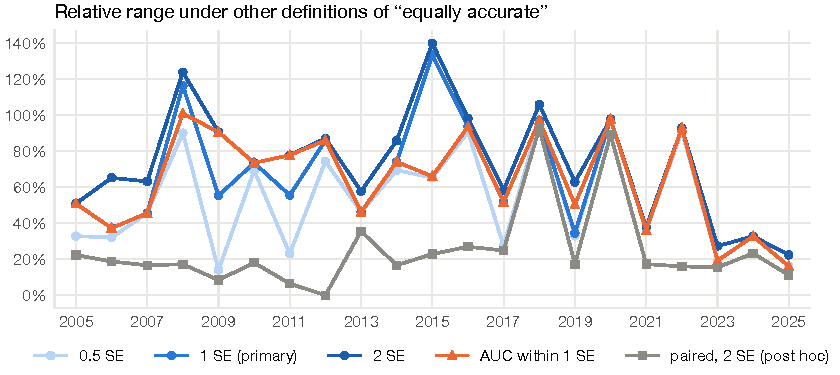
\includegraphics[width=\linewidth]{figures/sensitivity.pdf}
\caption{Relative range of the allowance across the set under other
definitions of equal accuracy. ``Paired'' admits models within two bootstrap
standard errors of their paired difference in held-out log loss from the best
(added after the results).}
\label{fig:sensitivity}
\end{figure}

\subsection{Where loans disagree}

The loan-level spread is large even where the aggregate range is modest. For
each scored loan, \cref{fig:loans} takes the ratio of its largest to smallest
lifetime PD across the set. Taking the median loan's ratio at each date
and then the median across dates, it is between \num{res.loan.ratio.min} and
\num{res.loan.ratio.max} in every LTV and credit-score band, and it is largest for the safest loans (current LTV below
60\% and credit scores of 760 or more), whose PDs are smallest. In
percentage points the spread is largest for loans in negative equity.
Disagreement in a sum over two hundred thousand loans partly cancels, which
is why the portfolio range is narrower than the loan-level ranges.

\begin{figure}[t]
\centering
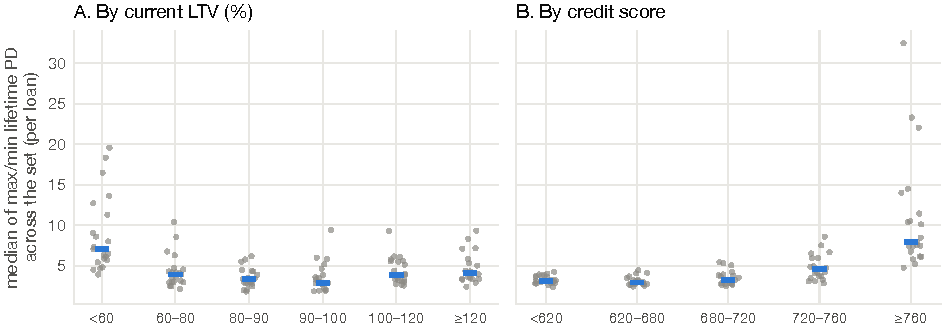
\includegraphics[width=\linewidth]{figures/loans.pdf}
\caption{Per loan, the ratio of the largest to the smallest lifetime PD
across the set; grey dots are the medians at each reporting date, the bar
the median across dates.}
\label{fig:loans}
\end{figure}
